%===============================================================================
% LaTeX sjabloon voor de bachelorproef toegepaste informatica aan HOGENT
% Meer info op https://github.com/HoGentTIN/bachproef-latex-sjabloon
%===============================================================================

\documentclass{bachproef-tin}

\usepackage{hogent-thesis-titlepage} % Titelpagina conform aan HOGENT huisstijl
\usepackage{listings}
\usepackage{hyperref}
\usepackage[utf8]{inputenc}
\usepackage{glossaries}
%%---------- Documenteigenschappen ---------------------------------------------
% TODO: Vul dit aan met je eigen info:

% De titel van het rapport/bachelorproef
\title{The headless usage of a traditional CMS to distribute centralised data}

% Je eigen naam
\author{Elan Goens}

% De naam van je promotor (lector van de opleiding)
\promotor{Lotte Van Steenberghe}

% De naam van je co-promotor. Als je promotor ook je opdrachtgever is en je
% dus ook inhoudelijk begeleidt (en enkel dan!), mag je dit leeg laten.
\copromotor{Marek Tyczyński}

% Indien je bachelorproef in opdracht van/in samenwerking met een bedrijf of
% externe organisatie geschreven is, geef je hier de naam. Zoniet laat je dit
% zoals het is.
\instelling{Dropsolid}

% Academiejaar
\academiejaar{2021-2022}

% Examenperiode
%  - 1e semester = 1e examenperiode => 1
%  - 2e semester = 2e examenperiode => 2
%  - tweede zit  = 3e examenperiode => 3
\examenperiode{2}


%===============================================================================
% Glossary entries
%===============================================================================


\newglossaryentry{CMS}
{
	name=CMS,
	description={A CMS or Content Management System is a piece of software that can help create and manage any content on a website}
}

\newglossaryentry{Drupal}
{
	name=Drupal,
	description={An open source CMS written in PHP, created by Dries Buytaert in 2001}
}

\newglossaryentry{PHP}
{
	name=PHP,
	description={A scripting or programming language often used in web development}
}

\newglossaryentry{Wordpress}
{
	name=Wordpress,
	description={An open source CMS written in PHP, created by Matt Wullenweg and Mike Little in 2003}
}

\newglossaryentry{Joomla}
{
	name=Joomla,
	description={An open source CMS written in PHP, created by Open Source Matters, Inc. in 2003}
}

\newglossaryentry{Headless}
{
	name=Headless,
	description={The practice of decoupling the front-end from the back-end of a CMS}
}

\newglossaryentry{Drupal core}
{
	name={Drupal core},
	description={The core release of Drupal, containing its most basic features}
}

\newglossaryentry{Composer}
{
	name={Composer},
	description={The dependency manager used for PHP}
}

\newglossaryentry{CLI}
{
	name={CLI},
	description={Command Line Interface, a way of interacting with a computer program through the use of text}
}

\newglossaryentry{NPM}
{
	name={NPM},
	description={Node Package Manager, the dependency manager used for JavaScript}
}

\newglossaryentry{OOP}
{
	name={OOP},
	description={Object Oriented Programming, a way of programming where objects are created that usually represent things that exist in real life}
}

\newglossaryentry{Node.js}
{
	name={Node.js},
	description={A JavaScript runtime environment}
}

\makenoidxglossaries


%===============================================================================
% Inhoud document
%===============================================================================

\begin{document}

%---------- Taalselectie -------------------------------------------------------
% Als je je bachelorproef in het Engels schrijft, haal dan onderstaande regel
% uit commentaar. Let op: de tekst op de voorkaft blijft in het Nederlands, en
% dat is ook de bedoeling!

\selectlanguage{english}

%---------- Titelblad ----------------------------------------------------------
\inserttitlepage

%---------- Samenvatting, voorwoord --------------------------------------------
\usechapterimagefalse
%%=============================================================================
%% Voorwoord
%%=============================================================================

\chapter*{\IfLanguageName{dutch}{Woord vooraf}{Preface}}
\label{ch:voorwoord}

%% TODO:
%% Het voorwoord is het enige deel van de bachelorproef waar je vanuit je
%% eigen standpunt (``ik-vorm'') mag schrijven. Je kan hier bv. motiveren
%% waarom jij het onderwerp wil bespreken.
%% Vergeet ook niet te bedanken wie je geholpen/gesteund/... heeft

Before you lies the bachelor's thesis “The headless usage of a traditional CMS to distribute centralised data". It has been written to fulfill the graduation requirements of the Applied Computer Science program at HogeSchool Gent (HoGent), with the specialization Mobile and Enterprise Developer.

As I am extremely interested in Content Management System as well as JavaScript frameworks, I wanted to do this research to extend my knowledge of these two subjects.

I want to thank my co-promotor Marek Tyczyński for always being available to give me feedback and answer my questions. Next to Marek, I could also count on the help of other employees of Dropsolid who are also excited about headless.

I also want to thank my promotor Lotte Van Steenberghe for giving me feedback about the structure of this thesis.

I want to thank my parents and my grandfather, who always supported and motivated me to keep going.

Finally I want to thank my girlfriend Emma, who is always by my side to support me.




%%=============================================================================
%% Samenvatting
%%=============================================================================

% TODO: De "abstract" of samenvatting is een kernachtige (~ 1 blz. voor een
% thesis) synthese van het document.
%
% Deze aspecten moeten zeker aan bod komen:
% - Context: waarom is dit werk belangrijk?
% - Nood: waarom moest dit onderzocht worden?
% - Taak: wat heb je precies gedaan?
% - Object: wat staat in dit document geschreven?
% - Resultaat: wat was het resultaat?
% - Conclusie: wat is/zijn de belangrijkste conclusie(s)?
% - Perspectief: blijven er nog vragen open die in de toekomst nog kunnen
%    onderzocht worden? Wat is een mogelijk vervolg voor jouw onderzoek?
%
% LET OP! Een samenvatting is GEEN voorwoord!

%%---------- Nederlandse samenvatting -----------------------------------------
%
% TODO: Als je je bachelorproef in het Engels schrijft, moet je eerst een
% Nederlandse samenvatting invoegen. Haal daarvoor onderstaande code uit
% commentaar.
% Wie zijn bachelorproef in het Nederlands schrijft, kan dit negeren, de inhoud
% wordt niet in het document ingevoegd.

\IfLanguageName{english}{%
\selectlanguage{dutch}
\chapter*{Samenvatting}

\selectlanguage{english}
}{}

%%---------- Samenvatting -----------------------------------------------------
% De samenvatting in de hoofdtaal van het document

\chapter*{\IfLanguageName{dutch}{Samenvatting}{Abstract}}

\lipsum[1-4]


%---------- Inhoudstafel -------------------------------------------------------
\pagestyle{empty} % Geen hoofding
\tableofcontents  % Voeg de inhoudstafel toe
\cleardoublepage  % Zorg dat volgende hoofstuk op een oneven pagina begint
\pagestyle{fancy} % Zet hoofding opnieuw aan

%---------- Lijst figuren, afkortingen, ... ------------------------------------

% Indien gewenst kan je hier een lijst van figuren/tabellen opgeven. Geef in
% dat geval je figuren/tabellen altijd een korte beschrijving:
%
%  \caption[korte beschrijving]{uitgebreide beschrijving}
%
% De korte beschrijving wordt gebruikt voor deze lijst, de uitgebreide staat bij
% de figuur of tabel zelf.

\listoffigures
%\listoftables
%\lstlistoflistings

% Als je een lijst van afkortingen of termen wil toevoegen, dan hoort die
% hier thuis. Gebruik bijvoorbeeld de ``glossaries'' package.
% https://www.overleaf.com/learn/latex/Glossaries

\clearpage
\printnoidxglossaries

%---------- Kern ---------------------------------------------------------------

% De eerste hoofdstukken van een bachelorproef zijn meestal een inleiding op
% het onderwerp, literatuurstudie en verantwoording methodologie.
% Aarzel niet om een meer beschrijvende titel aan deze hoofstukken te geven of
% om bijvoorbeeld de inleiding en/of stand van zaken over meerdere hoofdstukken
% te verspreiden!

%%=============================================================================
%% Inleiding
%%=============================================================================

\chapter{\IfLanguageName{dutch}{Inleiding}{Introduction}}
\label{ch:inleiding}

\section{Context}
A \gls{CMS}, or Content Management System, is, simply put, a piece of sofware that can be used create applications and manage the content used in these applications. There are two big use cases for a Content Management System: Enterprise Content Management (ECM), where the content managed is used in Enterprise applications, and Web Content Management (WCM), where the focus is on Web Applications and websites. The latter is the most common type. This type will also be the focus of this paper.

\gls{Drupal} is a free, open-source CMS written in \gls{PHP}. It was created in 2001 by Dries Buytaert, an open-source software developer. It is often seen as one of the most important players in the open-source web development community, and is widely used in websites and web applications around the world.

Many other CMSs exist, notable examples being \gls{Wordpress} and \gls{Joomla}. The choice to focus on Drupal stems from the fact that, in recent years, Drupal has evolved to be much more than a traditional CMS and has focused a lot more on communication with clients requesting data ~\autocite{So2018}. This is an important quality to have, considering how most users interact with content throught multiple different channels. For example, Facebook users can access the same content throught the web application, as throught the mobile app.

\gls{Headless} (or decoupled) is a concept that has been around for quite a while in the Drupal community, but it has started gaining some real traction the last couple of years. The headless usage of a CMS means that the back-end, the actual core of the CMS, is seperated from the integrated front-end it comes with. 

\section{\IfLanguageName{dutch}{Probleemstelling}{Problem Statement}}
\label{sec:probleemstelling}

Research into headless is getting more and more popular. Especially in the Drupal community, developers are realising the importance of modern front-end frameworks and tools and want to combine these with the CMS they know and love. 

Drupal, and other CMSs in general, are also going out of style at colleges and university. There is a severe lack of courses still teaching these subjects. Instead, there are more and more courses teaching modern javascript and mobile frameworks.


This is why it is so important to do research on headless. Businesses that are completely focussed on Drupal are already having a hard time recruiting young talent, and this will only get more difficult in the coming years. This paper can therefore be of vital importance to Dropsolid, to learn more about headless and how to effectively use it in new projects.

\section{\IfLanguageName{dutch}{Onderzoeksvraag}{Research question}}
\label{sec:onderzoeksvraag}

As already mentioned in section 1.1, this research will focus mainly on the usage and possibilities of headless Drupal. The main research question is:
\begin{itemize}
	\item In which situations would the usage of headless Drupal be advantageous?
\end{itemize}

Next to that there are a few supporting research questions:
\begin{itemize}
	\item What is needed to set up headless Drupal?
	\item Is headless a must-have, or a hype?
\end{itemize}

\section{\IfLanguageName{dutch}{Onderzoeksdoelstelling}{Research objective}}
\label{sec:onderzoeksdoelstelling}

This research will be a proof-of-concept to show what possibilities exist in the world of headless. The goal of this research is to give more insight into headless and how to use is, and to give some perspective to companies as to when to use this technology, and when not to.

\section{\IfLanguageName{dutch}{Opzet van deze bachelorproef}{Structure of this bachelor thesis}}
\label{sec:opzet-bachelorproef}

% Het is gebruikelijk aan het einde van de inleiding een overzicht te
% geven van de opbouw van de rest van de tekst. Deze sectie bevat al een aanzet
% die je kan aanvullen/aanpassen in functie van je eigen tekst.

The rest of this thesis will be constructed like this:

Chapter~\ref{ch:stand-van-zaken} will contain an overview of the basics of Drupal and a study of the possibilities headless Drupal has to offer.

Chapter~\ref{ch:methodologie} will discuss the methodology and will illustrate the ways in which headless Drupal will be tested in order to answer the research questions.

In chapter~\ref{ch:proofofconcept} the possibilities of headless Drupal will be studied closely and will be tested out. This will be done in a few different steps:

\begin{enumerate}
	\item Setting up a new Drupal website on a local environment
	\item Adding content to the Drupal website
	\item Exposing the content available on the Drupal website
	\item Consuming the exposed content with a front-end framework
\end{enumerate}

% TODO: Vul hier aan voor je eigen hoofstukken, één of twee zinnen per hoofdstuk

Lastly, in chapter~\ref{ch:conclusie}, a conclusion will be formulated based on what was discovered in chapter~\ref{ch:proofofconcept}. The research questions will also be answered, and this will be the starting point of any future research that has to be done on using a headless CMS.
\chapter{\IfLanguageName{dutch}{Stand van zaken}{State of the art}}
\label{ch:stand-van-zaken}

% Tip: Begin elk hoofdstuk met een paragraaf inleiding die beschrijft hoe
% dit hoofdstuk past binnen het geheel van de bachelorproef. Geef in het
% bijzonder aan wat de link is met het vorige en volgende hoofdstuk.

% Pas na deze inleidende paragraaf komt de eerste sectiehoofding.

As mentioned in the previous chapter, this research will go deeper into headless Drupal and attempt to figure out how to utilise it and why it became so popular. But before answering these questions it is important to have a clear understanding of what headless Drupal actually is. This will be discussed in this chapter. 

\section{Drupal: the basics}

Before diving into headless, a torough understanding of the CMS, in this is case Drupal, is required. This section will cover the basics of Drupal that are needed to get started with headless.

%%%%%%%%%%%%%%%%%%%%%%%%

\subsection{Drupal core}

When installing Drupal with the standard profile, only \gls{Drupal core} is included. Drupal core includes all the basic features you need to get started on a website. Some of the most important features that are included in core according to \textcite{Tomlinson2015} are: 

\begin{itemize}
	\item  content
	\item  menus
	\item  users
	\item  roles and permissions
	\item  views
\end{itemize}

For any basic site Drupal core will probably suffice, but often a feature is needed that is not included in core. That is when contributed (contrib) and custom modules come in handy \autocite{Tomlinson2015}.

%%%%%%%%%%%%%%%%%%%%%%%%%%%%%

\subsection{Contributed and custom modules}

Contributed modules are custom modules, made by developers in the Drupal community, that are free to use and completely open to customization. There are thousands of contributed modules available on \url{https://www.drupal.org}. Some examples of popular contributed modules according to \textcite{Tomlinson2015} are: 

\begin{itemize}
	\item  \emph{Commerce}
	\item  \emph{Display Suite}
	\item  \emph{Backup and Migrate}
	\item  \emph{Pathauto}
\end{itemize}

As said before, these contributed modules are all available and free to use on \url{https://www.drupal.org}. There is also the possibility for developers to create their own custom modules. For most things you would want for your site, you can probably find a contributed module, but sometimes those don't do exactly what you want. That's when you can create your own module, or customize one of the contributed modules to fit your needs.

\subsubsection{Composer}
\label{sss:composer}

When talking about contributed modules, it is important to also mention \gls{Composer}. According to \textcite{M.Kromann2018}, Composer is a dependency manager for the PHP programming language. As such, it can be used in Drupal project to easily install contributed modules from a \gls{CLI} (Command Line Interface). It can be compared to \gls{NPM} (Node Package Manager), which is a package manager for JavaScript. Installing contributed modules with composer is fairly simple. Simply running the "composer require {module name}", with "{module name}" replaced by the name of the module you want to install, will install this module. Enabling the module can then be done using the Drupal UI.

\subsection{Drush}

Drush is, according to \textcite{Tomlinson2015}, \emph{"a command line tool that greatly simplifies the tasks of building and administering a Drupal website."} Drush allows you to perform specific tasks related to your Drupal website, one of which is installing the website.

%%%%%%%%%%%%%%%%%%%%%%%%%%%%%

\subsection{The building blocks of Drupal 9}

Drupal 9 Core has a few fundamental concepts that make up the entirety of the system. This section will take a deeper look at these.

\subsubsection{Content and Content Types}

Content Types are, according to \textcite{Tomlinson2015}, often seen as the single most powerful feature Drupal has to offer. A content type is defined by ~\textcite{Drupal2021} as \emph{"a pre-defined collection of data types (Fields) which relate to each other by an informational context"}. In other words, a Content Type is a sort of template by which content can be created.

A standard Drupal 9 installation includes two basic content types to get you started: \emph{Basic page} and \emph{Article}. Other than these two, you can also create your own custom content type. Custom content types can be anything, but like in Object Oriented Programming (\gls{OOP}), they usually represent some real world object~\autocite{Tomlinson2015}.

\subsubsection{Blocks}
\label{sss:blocks}

\textcite{Drupal2021} defines blocks as \emph{"boxes of content rendered into an area, or region, of a web page"}. Drupal offers a few standard block included in Drupal core, but just like with content types it is possible to create your own custom blocks that can include any content available in the system. As the definition states, blocks can be placed inside of regions, on any page. This is done using the block layout manager, or by using Layout Builder \autocite{Tomlinson2015}. The latter will be discussed more in section \ref{sss:lb}.

\subsubsection{Users, Roles and Permissions}

For most websites nowadays, it is important to have the ability to control who can access the content on the site. For this purpose Drupal includes \emph{Users}. These users are seperated into two different groups~\autocite{Tomlinson2015}:
\begin{itemize}
	\item  Anonymous Users: These are Users that are not logged in to your site. These users often have restricted access to websites.
	\item  Authenticated Users: These are Users that log in to your site, generally using a combination of an email address and a password. Usually these users have access to all the functionalities the site has to offer.
\end{itemize}

\emph{Roles} are usually defined as categories. Each Autheticated User has a specific role assigned to them. Some roles have access to more part of the site than others. This allows you to completely control what you want specific Users to be able to do on your site~\autocite{Tomlinson2015}.

\emph{Permissions} are enabled or disabled on a specific role. These allow you to control what roles can do certain things on your site. For example, one role could have the permission to be able to edit certain pages, while another role does not~\autocite{Tomlinson2015}.

\subsubsection{Views}

Views is one of the most important, and also one of the most used modules in Drupal 9. It has been a part of Drupal Core since Drupal 8. The Views module allows you to create lists content that can be displayed on your website \autocite{DrupalViews}.

The concept of Views in Drupal 9 is realized in two modules: the core \emph{Views} module, and the \emph{Views UI} module accompanying it \autocite{DrupalViews}. Views UI offers an administration interface to work with and create views, so it is a crucial part of Views in its entirety~\autocite{Tomlinson2015}.

As already mentioned, in its simplest form Views allows you to create lists of content. But there are a lot of customization and configuration options available here. For example, there is the possibility to display your content in a regular list, but you can also choose to display it in a table, or even a grid~\autocite{Tomlinson2015}.

Views also offers the possibility to create multiple different displays for your lists. For example, you could display your view on a dedicated page, but you could also create a block for it, that you can then display on any page you like. Another feature available with Views, is the ability to sort or filter any lists you create~\autocite{Tomlinson2015}.

\subsubsection{Taxonomy}

Taxonomy in Drupal 9 is, according to~\textcite{Tomlinson2015}, a very underused feature. ~\textcite{MerriamWebsterTax} defines taxonomy as \emph{"the study of the general principles of scientific classification"}. Taxonomy in Drupal essentialy means the same thing. It is a way to classify certain things on your site.

According to~\textcite{Tomlinson2015}, taxonomy in Drupal is divided into two different groups: tagging and structured taxonomy. Tagging enables you to register key words on you site, and then assign that tag to some piece of content, essentially grouping it. This is useful to, for example, filter some content that is displayed in a list based on a specific tag. The big problem with this kind of classification is that it is easy to make mistakes that make the whole system difficult to use. For example, you could misspell a taxonomy term, making it harder for users to find content tagged with this tag, as they would not show up when searching for it~\autocite{Tomlinson2015}.

Structured taxonomy takes a different approach. With this approach, only the admin of the site can create taxonomy terms. You can then categorize content by simply choosing one or more of these terms when editing the content. This way users will only be able to filter the content based on those terms, but you also would not run into the issue interfering with the user experience by making a mistake while creating the terms. Another benefit of structured taxonomy is that it gives you the possibility to create a certain hierachy, meaning you can create groups of taxonomy terms, which then group some content together, giving you some more customization~\autocite{Tomlinson2015}.

%%%%%%%%%%%%%%%%%%%%%%%%%%%%%

\subsection{The front-end}

The Drupal Content Management System includes a front-end functionality that can be used to display data. In this section, some of the most important concepts of the Drupal front-end will be discussed.

\subsubsection{Themes}

Themes are used within Drupal to change the look and feel of the website and are made up of Hypertext Markup Language (HTML) and Cascading Style Sheets (CSS). According to ~\textcite{Tomlinson2015}, a Drupal theme defines four main components on a Drupal website: 

\begin{itemize}
	\item  The colors used
	\item  The fonts used
	\item  The placement of images and graphics
	\item  The layout of a page
\end{itemize}

The default theme that is installed on any new Drupal website is the Bartik theme. Other themes, like contributed modules, are available to use on \url{https://www.drupal.org}. Drupal 9 allows you to choose different themes for the site itself and for the administration portion of the site. Many of the available themes use the same, or at least a very similar layout to the default theme, but Drupal also gives you the possibility to customize any of these themes or even lets you create your own theme~\autocite{Tomlinson2015}.

A Drupal theme usually consists of multiple regions, in which content and blocks can be placed. These regions can be customized to fit your needs. Commonly used regions include~\autocite{Tomlinson2015}: 
\begin{itemize}
	\item  Menus, allowing for the placements of links and menu items
	\item  Sidebars
	\item  Headers
	\item  Footers
	\item  A content region that is usually the main region of a page and allows the placement of any content
\end{itemize}

\begin{figure}
	\centering
	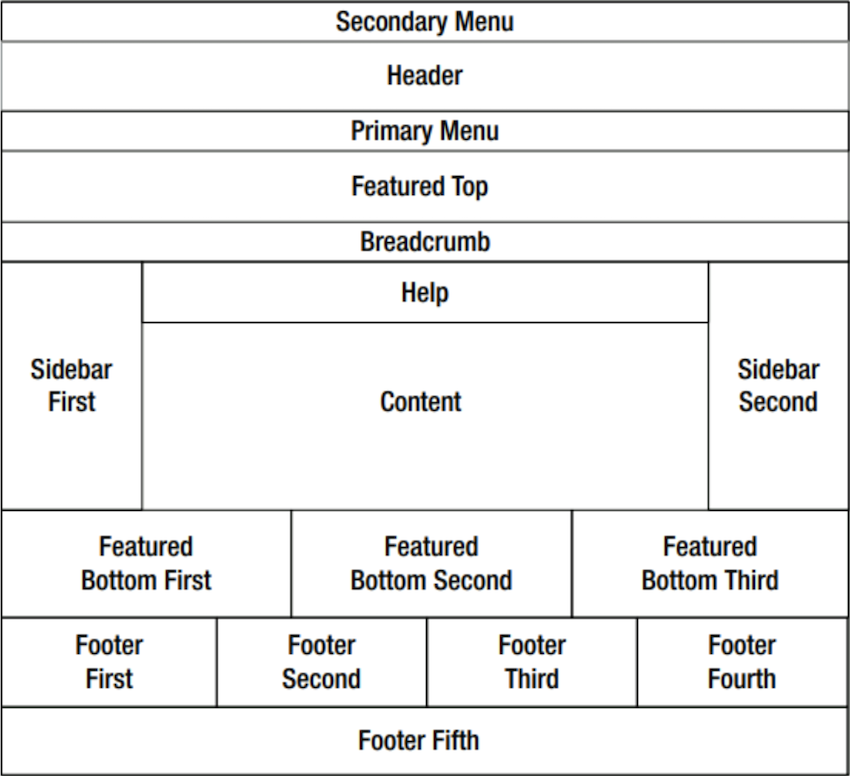
\includegraphics{./img/Bartik_Theme.png}
	\caption[The Bartik theme]{A representation of the layout used by the default Bartik theme ~\autocite{Tomlinson2015}}
\end{figure}


\subsubsection{Layout Builder}
\label{sss:lb}

Before the introduction of Drupal 8 theming and styling your website tended to be a little tedious. However, with Drupal 8 came a new feature to make managing the front-end of your website a little easier and more straight forward: Layout Builder~\autocite{Drupal2021}.

Layout Builder is a tool that allows you to create layouts using a visual drag and drop interface. It allows you to easily place any blocks on your pages within the regions provided by your theme, and also lets you display any piece of content. The useful thing about Layout Builder is that it can be used by people without much technical knowledge, as there is no need to write any code. Previously, other tools like \emph{Display Suite} and \emph{Panels} were used to accomplish this kind of thing. The problem here was that these modules were, in many cases, incompatible with one another~\autocite{Drupalize2022}.

When creating a layout using Drupal Layout Builder, two main concepts are used~\autocite{Drupalize2022}: 
\begin{itemize}
	\item  Sections are containers in which blocks can be placed.
	\item  Blocks are any kind of content, and can be placed within any section.
\end{itemize}
There is a difference between the blocks specific to Layout Builder and the Drupal blocks which were mentioned in section \ref{sss:blocks}. The blocks used in Layout Builder are considered to be more of a guideline, or a placeholder indicating where some specific piece of content goes~\autocite{Drupalize2022}.




%%%%%%%%%%%%%%%%%%%%%%%%%%%%%

\section{Architectures}
A traditional CMS like Drupal in its base form consists of a monolithic architecture. This means that the CMS offers anything a user would need in a web application, including a database, back-end and front-end.

When going headless, the architecture of the CMS goes from monolithic to the so-called decoupled architecture. In this form, only the back-end and database that the CMS offers are utilised. Then, instead of distributing the content in this back-end to one channel, it can be consumed by different channels, including web applications made with front-end frameworks like React and Angular, but even mobile applications.

Monolithic and decoupled are the two main architectures that are considered when using a CMS, but there are two other architectures worth mentioning: the fully decoupled static site and progressively decoupled ~\autocite{Dropsolid2021}. The latter two are less well known, but are still important to look at to get the whole picture of what headless is. All of these architectures will be discussed in this chapter.

%%%%%%%%%%%%%%%%%%%%%%%%%%%%%

\subsection{Monolithic or Traditional}
The traditional or monolithic architecture is the one used by all traditional CMSs out of the box. It means that the application is one big end-to-end system. For Drupal in particular, this means that the theming functions which encompass the front-end are completely coupled and dependent on Drupal's back-end.

This architecture has both upsides and downsides. One big upside is that this is a very robust and reliable system. The system is predictable and easy to use. The downside to this architecture is that it has led to something often called Drupalisms on the front-end ~\autocite{So2018}. This means that some terminology and features specific to Drupal came to exist, which are hard to understand for developers less familiar with Drupal. 

One other negative is that this system can feel limiting for front-end developers, because they have to work within the boundaries of the specific theme they are using.

\begin{figure}
\centering
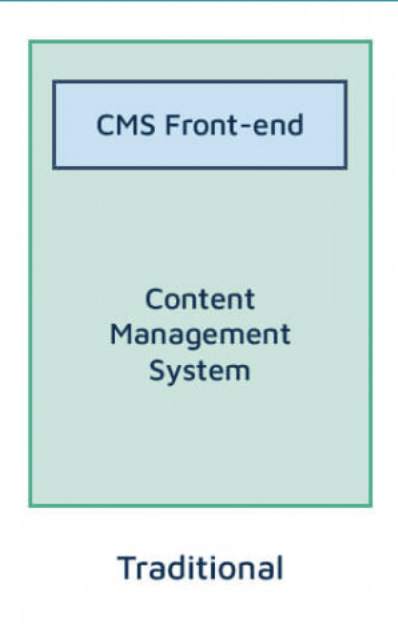
\includegraphics{./img/Traditional_Architecture}
\caption[Traditional CMS architecture]{A representation of the traditional or monolithic architecture ~\autocite{Dropsolid2021}}
\end{figure}

%%%%%%%%%%%%%%%%%%%%%%%%%%%%%

\subsection{Headless or Decoupled}

The fully decoupled or headless architecture is the one that has become more and more popular over the years ~\autocite{Dropsolid2021}. Decoupled means that the components of the system don't depend on each other like they do with the monolithic architecture ~\autocite{So2018}. They interact with each other using web services instead.

Fully decoupling the back-end from the front-end is the most well known type of decoupled out there. It allows developers much more freedom to choose any technology they want to build the presentation layer (front-end) of the application.

This approach is the one that will be discussed further in this research.

\begin{figure}
	\centering
	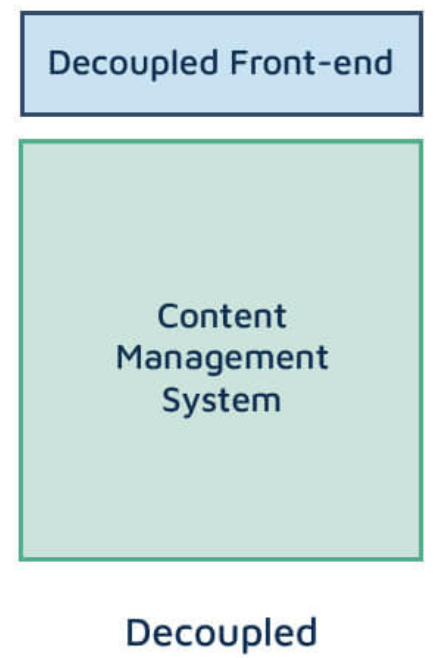
\includegraphics{./img/Headless_Architecture}
	\caption[Headless CMS architecture]{A representation of the decoupled or headless architecture ~\autocite{Dropsolid2021}}
\end{figure}

%%%%%%%%%%%%%%%%%%%%%%%%%%%%%

\subsection{Fully decoupled static site}

The main difference this architecture has with the previous one is that content is not stored by the CMS itself. The content is instead maintained inside the front-end framework that is used. This is done using Hypertext Markup Language (HTML), Cascading Stylesheets (CSS) and Javascript (JS) files ~\autocite{Dropsolid2021}.

The big advantage of this approach is that performance and security are segnificantly enhanced, while also reducing the complexity for developers.

The approach with this kind of architecture is generally consists of retrieving content from the CMS with a static site generator, after which the static website is deployed to a Content Delivery Network (CDN) which, according to ~\textcite{Buyya2008}, is a "collaborative collection of network elements spanning the Internet, where content is replicated over
several mirrored Web servers in order to perform transparent and effective delivery of content to the end users".

%%%%%%%%%%%%%%%%%%%%%%%%%%%%%

\subsection{Progressively decoupled}

When using a progressively decoupled approach, the back-end of the CMS is not completely decoupled from the front-end. Instead, a javascript front-end framework is integrated, interwoven into the existing CMS front-end. This means that the Drupal front-end is still kept and not entirely replaced, unlike in the other two decoupled approaches~\autocite{So2018}. 

\begin{figure}
	\centering
	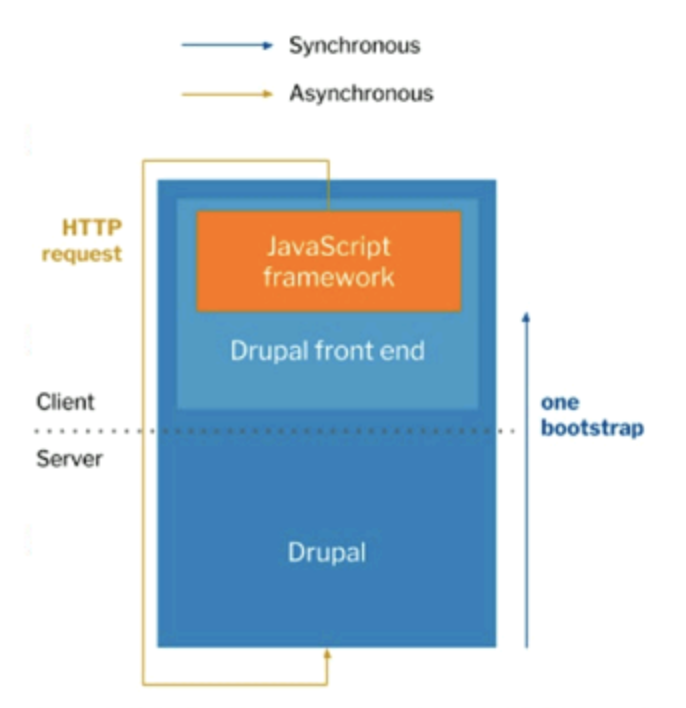
\includegraphics{./img/Progressively_Decoupled.png}
	\caption[Progressively decoupled CMS architecture]{A representation of the progressively decoupled architecture ~\autocite{So2018}}
\end{figure}

%%%%%%%%%%%%%%%%%%%%%%%%%%%%%

\section{RESTful Web Services}

%%%%%%%%%%%%%%%%%%%%%%%%%%%%%

\subsection{Basics of REST}
Representational State Transfer or REST is, according to~\textcite{Wilde2011}, \emph{"A set of constraints that inform the design of a hypermedia system"}. It is an architectural style with a set of guiding principles. The main principles are: 
\begin{enumerate}
	\item Uniform Interface: All interactions are to be made around an interface that supports all these interactions.
	\item  Stateless: All interactions between a client and server need to be independent from one another.
	\item Client-Server: User-interface or client concerns are to be seperated strictly from back-end and data, or server related concerns.
	\item Layered System: Seperate components should not be allowed to see any layer beyond the layer they are interacting with.
	\item Caching: Any resources should allow for caching by the client, the server and any other components.
\end{enumerate}

\begin{figure}
	\centering
	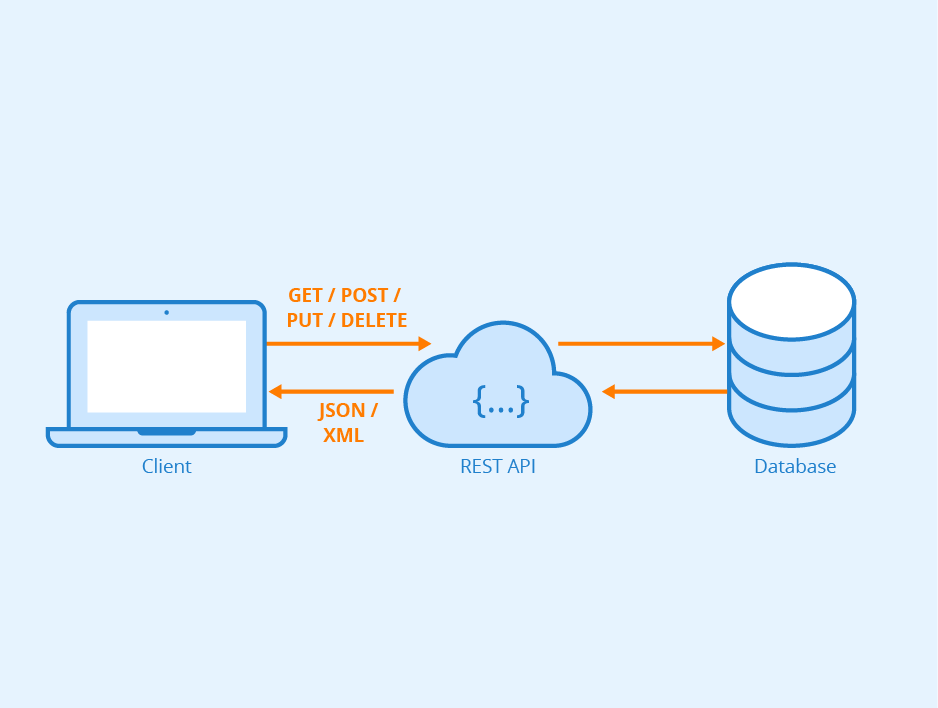
\includegraphics{./img/Rest-API.png}
	\caption[REST API]{A representation of a REST API ~\autocite{Seobility}}
\end{figure}

%%%%%%%%%%%%%%%%%%%%%%%%%%%%%

\subsection{Web services in Drupal 9}
Within Drupal 9 there exist two main ways of going headless. The most straightforward of the two is the JSON:API module. The other, which requires more configuration, is the Drupal core RESTful web services module~\autocite{Drupal2018}. 

Both of these modules provide the possibility to interact with data through the classic HTTP request methods. According to~\autocite{Wilde2011} these methods are: 

\begin{itemize}
	\item GET: requests the retrieval of specific data.
	\item POST: requests the creation of some data, which is usually defined in the body of the request.
	\item PUT/PATCH: requests that some data is updated. The data to be updated is usually identified by its id, and the new data is normally defined in the body of the request like with a POST method.
	\item DELETE: requests the deletion of specific data.
\end{itemize}

\subsubsection{JSON:API}
\label{sss:JSONAPI}

Before the release of Drupal 8, the JSON:API was an immensly popular web services contributed module. Due to it's popularity and wide use, the first stable release of the module was included in Drupal core in Drupal 8.7. This meant that anyone using Drupal from that point on could easily enable the module on any Drupal installation. The only requirement for this module to be enabled is that the Serialization module also has to be enabled~\autocite{Drupal2019}.

This module is meant to be easy to use, without a lot of configuration being necessary. Enabling the module will give the developer access to a REST API for any content type available on the website, exposing all the content of those types~\autocite{So2018}. This approach has many advantages. The main advantage is that is is very easy to use. One click is all it takes to enable the module and make all relational data available~\autocite{So2018}.

On the other hand, exposing all data like this this also means that, in a lot of situations, a lot of data will be exposed that won't ever be used because it is not needed. There is no in between with this module: you enable it and expose all data, or don't enable it and expose no data at all~\autocite{So2018}.

Using this module, the data of each entity is exposed in a set structure, using two members inside the JSON object. The \emph{attributes} member holds all data that is specific to that entity, like a name or a birthdate for an entity representing a person~\autocite{Drupal2019}. 

The \emph{relationships} member holds a limited amount of data of another entity with which the current entity has some kind of relationship. An example of this would be when a \emph{person} entity has a relationship with a \emph{house} entity, the title and id of that house would be available under the relationships of that person~\autocite{Drupal2019}.

As said earlier this module does not require any configuration. The only configuration option that is available out of the box, is the option to only accept read (GET) operations, or to also allow create (POST), update (PUT/PATCH) and delete (DELETE) operations~\autocite{So2018}.


\subsubsection{RESTful web services}

Another option to expose data in Drupal 9 is the RESTful web services module. This module has been included in Drupal core since Drupal 8. Just like the JSON:API module it depends on the Serialization module to work~\autocite{Drupal2018}.
This module generally considered harder to use than the JSON:API module. This is because this module does not work out of the box like JSON:API does. It requires quite a bit of configuration to get it working~\autocite{Drupal2018}.

The compexity of this module has some cons, but also some pros. The big advantage this module offers compared to the JSON module, is that it allows the developer to pick and choose the resources and content types to be made available. It can be customized so that only one content type is exposed, while the JSON:API module only allows you to expose all content types within the system~\autocite{So2018}. 

But with this customizability comes a cost. To make this module work, the developer has to configure each entity type they want exposed seperately. This can be a very tedious task, especialy in bigger sites where tens, if not hundreds of entity types can exist.

The big difference between this module and the previous one, is that with the REST module data other than entities can be exposed through the creation of custom RestResource plugins. This means that it offers the possibility of exposing any custom data that might exist within the system. An example of this would be some piece of configuration.

For most use cases however, just being able to expose entities will be more than enough. This is why this module has lost some popularity in recent years in favor of JSON:API~\autocite{So2018}.


\section{Front-end possibilities with headless}

As illustrated in the last section, there are multiple possibilities to expose data in Drupal 9. Data that is exposed can be consumed by any front-end technology that has some sort of way to handle HTTP requests. In this section some of these technologies will be discussed.

\subsection{Web applications}

When it comes to consuming data from an external API, the JavaScript front-end frameworks have been king for the last few years. They allow developers to easily make a request to a URL. One of the biggest players in this field is Angular. Being backed by Google, it means Angular has a very active community of developers around it. Other examples of JavaScript frameworks include the also well known React and Vue.js. Another less well known example is Svelte, a framework that has been gaining a lot of traction in the last couple of years~\autocite{Uzayr2019}.

\subsubsection{Angular components}

According to \textcite{Freeman2020}, Angular components are the main building blocks of an Angular application. A component consists of:

\begin{itemize}
	\item An HTML template
	\item A TypeScript class
	\item A CSS selector
	\item A CSS file that applies only to this HTML template
\end{itemize}



\subsubsection{Angular dependency injection}

\subsubsection{Angular Observables}

Angular makes use of a concept called \emph{Observables} to handle various asynchonous tasks, like getting data form a server. Observables can be described as a kind of "container" that contains some data. An observable can be subscribed to in order to receive the data that is contained within. The interesting thing about observables is that when any data in the observable changes, any subscribers are notified of this so they can immediately receive the new data.

\subsection{Mobile applications}
%%=============================================================================
%% Methodologie
%%=============================================================================

\chapter{\IfLanguageName{dutch}{Methodologie}{Methodology}}
\label{ch:methodologie}

%% TODO: Hoe ben je te werk gegaan? Verdeel je onderzoek in grote fasen, en
%% licht in elke fase toe welke stappen je gevolgd hebt. Verantwoord waarom je
%% op deze manier te werk gegaan bent. Je moet kunnen aantonen dat je de best
%% mogelijke manier toegepast hebt om een antwoord te vinden op de
%% onderzoeksvraag.




% Voeg hier je eigen hoofdstukken toe die de ``corpus'' van je bachelorproef
% vormen. De structuur en titels hangen af van je eigen onderzoek. Je kan bv.
% elke fase in je onderzoek in een apart hoofdstuk bespreken.

%%=============================================================================
%% Methodologie
%%=============================================================================

\chapter{\IfLanguageName{dutch}{Proof of Concept}{Proof of Concept}}
\label{ch:proofofconcept}

\section{Setting up a new Drupal 9 site}

Creating a new Drupal 9 site with the standard Drupal 9 profile on a local server environment is fairly simple. Some different steps are involved depending on the Operting System, but overall the workflow goes like this: 
\begin{itemize}
	\item Create a local environment using an AMP (Apache HTTP server, MySQL relational database, PHP programming language) stack. On the most popular OSs, Linux, Windows and MacOS, packages are available that include all of these technologies. These allow for a smooth and simple process of installing a local environment.
	\item Installing Drupal. The latest release of Drupal can always be found on the Drupal.org site.
\end{itemize}

\section{Exposing data}

At the basis of using a headless CMS lies the exposing of data. This means that the data that is available within the CMS is exposed through the use of a file format like JSON or XML, just like it would be done in a traditional web API. When correctly configured, any source can then ask for and receive that data, after which they can do with it as they like. Data can also be sent back to the CMS by client applications. In Drupal 9 there are two main modules that fulfill this purpose: JSON:API and RESTful Web Services.

\subsection{The JSON:API module}

\subsection{The  RESTful Web Services module}

\section{The front-end}

\subsection{Single page web application with Angular}

\subsection{Mobile application with SwiftUi}
%\input{...}
%...

%%=============================================================================
%% Conclusie
%%=============================================================================

\chapter{\IfLanguageName{dutch}{Conclusie}{Conclusion}}
\label{ch:conclusie}

% TODO: Trek een duidelijke conclusie, in de vorm van een antwoord op de
% onderzoeksvra(a)g(en). Wat was jouw bijdrage aan het onderzoeksdomein en
% hoe biedt dit meerwaarde aan het vakgebied/doelgroep? 
% Reflecteer kritisch over het resultaat. In Engelse teksten wordt deze sectie
% ``Discussion'' genoemd. Had je deze uitkomst verwacht? Zijn er zaken die nog
% niet duidelijk zijn?
% Heeft het onderzoek geleid tot nieuwe vragen die uitnodigen tot verder 
%onderzoek?




%%=============================================================================
%% Bijlagen
%%=============================================================================

\appendix
\renewcommand{\chaptername}{Appendix}

%%---------- Onderzoeksvoorstel -----------------------------------------------

\chapter{Onderzoeksvoorstel}

Het onderwerp van deze bachelorproef is gebaseerd op een onderzoeksvoorstel dat vooraf werd beoordeeld door de promotor. Dat voorstel is opgenomen in deze bijlage.

% Verwijzing naar het bestand met de inhoud van het onderzoeksvoorstel
%---------- Inleiding ---------------------------------------------------------

\section{Introductie} % The \section*{} command stops section numbering
\label{sec:introductie}

Een CMS (Content Management Systeem) is een 
webapplicatie die mensen met weinig technische kennis de mogelijkheid geeft content te publiceren op de applicatie. De oorsprong van deze systemen ligt in de jaren '90, wanneer bedrijven als FileNet en Storybuilder closed source systemen ontwikkelden. Pas tien jaar later, in de vroege jaren 2000, ontstonden de eerste open source alternatieven zoals Drupal en Wordpress. Dit zijn systemen die de dag van vandaag nog altijd heel populair zijn. ~\autocite{Burgy2020}

Content management systemen hebben heel wat voordelen, zoals gemak van gebruik en snelheid van ontwikkeling. Ze brengen echter ook een paar grote beperkingen met zich mee. Zo hangt de front-end van de applicatie helemaal vast aan de back-end, wat ervoor zorgt dat de applicatie minder flexibel is. In een tijd waarin microservices meer en meer belangrijk worden ~\autocite{Shabani2021}, is het dan ook belangrijk dat CMS mee evolueren.

Het gebruiken van een headless CMS kan deze problemen oplossen. Hier worden namelijk de back-end en de front-end losgekoppeld van elkaar. Dit geeft de ontwikkelaar meer flexibiliteit, maar hierbij gaan enkele belangrijke features van de CMS, waaronder SEO en het gebruik van thema's verloren. Ook draait de ontwikkeling vaak duurder uit. ~\autocite{Luksza}

Doordat het gebruik van een headless CMS meer en meer populair wordt ~\autocite{Luksza} is het belangrijk om te analyseren wat precies de gevolgen zijn hiervan. Hoe kan een headless CMS worden gebruikt? Hoe zet je een headless Drupal site op? In welke situaties zou het gebruik van headless een voordeel kunnen opleveren? Op deze vragen zal in dit onderzoek een antwoord worden gegeven.




%---------- Stand van zaken ---------------------------------------------------

\section{State-of-the-art}
\label{sec:state-of-the-art}

\subsection{Wat is een CMS}
Een CMS, voluit Content Management Systeem, is een webapplicatie die mensen met weinig technische kennis de mogelijkheid geeft content te publiceren op de applicatie. Deze systemen worden al jarenlang gebruikt, en bieden tal van voordelen tegenover de traditionele ontwikkeling van webapplicaties.

\subsection{Wat is headless}
Bij headless wordt, zoals de naam al doet vermoeden, het 'hoofd' van het 'lichaam' van de CMS gescheden. Dit zorgt ervoor dat je alleen de back-end van de applicatie overhoudt. Dit maakt het mogelijk om meerdere applicaties hiermee te verbinden die allemaal dezelfde, gecentraliseerde content gebruiken en presenteren. 

Zo kan je bijvoorbeeld een webapplicatie schrijven in een framework als React, maar ook native applicaties geschreven voor IOS of Android kunnen hier gebruik van maken. Dit is dan ook het grootste voordeel van deze aanpak: al de data is gecentraliseerd op een plek. Dit kan je ook bereiken door zelf een API te schrijven, maar dan verlies je de voordelen die een moderne CMS met zich meebrengt, en dan vooral dat mensen met weinig technische kennis ook de content kunnen  bewerken. 

In een vergelijkende studie van ~\autocite{Barker2018} wordt aangetoond welke factoren er belangrijk zijn in de keuze voor een headless CMS. Zo wordt er bijvoorbeeld gesproken over Content Modeling. Dit is eigenlijk de basisfunctie van elk CMS: het weergeven van content en data op een beheerbare manier. Hiervoor wordt in de meeste gevallen gebruik gemaakt van Content Types. Er bestaan drie verschillende manieren om dit te modelleren: discreet, relationeel, en organisationeel.

\subsection{Search Engine Optimisation}
SEO of Search Engine Optimisation is de kunst om webverkeer en webgebruikers naar een website te leiden ~\autocite{Davis2006}. In praktisch alle moderne Content Management Systems zijn er plugins of tools aanwezig die helpen om dit proces te optimaliseren. In Wordpress zijn er bijvoorbeeld meer dan 85 plugins die zich hiermee bezig houden ~\autocite{Juliao2020}. 

Wat er volgens ~\autocite{Shreves2012} ook heel erg belangrijk is voor SEO zijn keywords die zich bevinden in de domeinnaam en op de pagina's van een website. Hier moet dus ook zeker rekening mee gehouden worden.

\subsection{Belang van dit onderzoek}
Het belang van dit onderzoek is dat er hier ook zal gefocust worden op de workflow die ontwikkelaars moeten doorlopen om een CMS headless te gebruiken. Ook zal er bekeken worden wat de invloed is op SEO wanneer een headless CMS wordt gebruikt, iets wat nog weinig onderzocht is. 

De meeste bestaande onderzoeken naar headless CMS zijn vergelijkend, en vergelijken dus verschillende CMS met elkaar met als doel de beste keuze te bepalen ~\autocite{Barker2018}. Dit onderzoek zal eerder dieper ingaan op hoe een headless CMS in zijn werk gaat en wat de voordelen en nadelen ervan zijn ten opzichte van een traditioneel systeem.

% Voor literatuurverwijzingen zijn er twee belangrijke commando's:
% \autocite{KEY} => (Auteur, jaartal) Gebruik dit als de naam van de auteur
%   geen onderdeel is van de zin.
% \textcite{KEY} => Auteur (jaartal)  Gebruik dit als de auteursnaam wel een
%   functie heeft in de zin (bv. ``Uit onderzoek door Doll & Hill (1954) bleek
%   ...'')

Je mag gerust gebruik maken van subsecties in dit onderdeel.

%---------- Methodologie ------------------------------------------------------
\section{Methodologie}
\label{sec:methodologie}

Er zal in dit onderzoek eerst en vooral bekeken worden welke opties er bestaan voor het gebruiken van een headless CMS en hoe dit kan worden opgezet. Ook zal er worden onderzocht hoe je een traditioneel CMS omzet naar een headless CMS.

Daarnaast zal er ook worden onderzocht wat de gevolgen zijn van het gebruik van een headless CMS ten opzichte van een traditioneel. Er zal dus besproken worden wat de voor - en nadelen zijn hiervan, en voor wie welke optie het meest geschikt is. De snelheid van ontwikkelen zal worden gemeten in beide gevallen.

Als laatste wordt er ook onderzocht hoe SEO precies werkt binnen een traditioneel CMS en binnen headless. Hier wordt bekeken of er grote verschillen zijn tussen de twee opties. Ook andere features die in een traditioneel systeem aanwezig zijn, zoals thema's, zullen worden bekeken en er zal worden onderzocht of deze een groot tijdsvoordeel opleveren bij de ontwikkeling.

Deze dingen zullen worden gemeten door verschillende systemen te gebruiken, zowel traditioneel als headless. Hierna kan er een vergelijking worden gemaakt over hoeveel tijd de ontwikkeling in beslag neemt, en welke features een voordeel opleveren wat betreft ontwikkelingssnelheid. De SEO zal worden geanalyseerd door middel van bestaande sites, gebruik makende van Google analytics en tools inbegrepen in de CMS zelf. De resultaten hiervan zullen worden vergeleken met elkaar.

%---------- Verwachte resultaten ----------------------------------------------
\section{Verwachte resultaten}
\label{sec:verwachte_resultaten}

Het headless gebruik van een traditionele CMS kan best wel wat tijd in beslag nemen. Zo moeten er REST endpoints worden opgemaakt om de data beschikbaar te stellen voor de losgekoppelde front-end. 

Er wordt verwacht dat het ontwikkelen van een headless webapplicatie een stuk meer tijd zal innemen dan bij het gebruik van een traditionele CMS, maar de flexibiliteit en de personaliseerbaarheid zal hier wel veel beter zijn. Ook zullen de SEO optimalisaties die inbegrepen zijn in een standaard CMS verloren gaan, waardoor deze door de developer zelf nog zullen moeten gebeuren.


%---------- Verwachte conclusies ----------------------------------------------
\section{Verwachte conclusies}
\label{sec:verwachte_conclusies}

De populariteit van Content Management Systemen zal blijven groeien. Zeker headless CMS is een technologie die meer en meer gebruikt zal worden. De flexibiliteit die je krijgt door het opsplitsen van back - en front-end is voor ontwikkelaars extreem waardevol. Headless is echter geen vervanging voor een traditionele CMS en dat zal het waarschijnlijk ook nooit worden. 



%%---------- Andere bijlagen --------------------------------------------------
% TODO: Voeg hier eventuele andere bijlagen toe
%\input{...}

%%---------- Referentielijst --------------------------------------------------

\printbibliography[heading=bibintoc]

\end{document}
